\chapter{From Newton's formulae to B-splines}\label{chapter1}

\section{``Classical'' interpolation theory}\label{sec:classical} 

The age of scientific revolution, spanning from early 17th to late 19th century, brought invaluable scientific knowledge 
in all domains including the mathematics with the contributions of the likes of Descartes, Leibniz, Newton, Euler, 
Lagrange, Gauss and many others. This era saw the development of new theories and tools that laid the foundations for 
modern mathematics as we know them. In particular, new techniques were devised for interpolating between a given set of 
points, a problem that can be traced back to ancient times. As a matter of fact, interpolation was already in use in 
ancient Babylon where farmers were concerned with predictions about astronomical events as the positions of the sun, 
moon and known planets.  Lists recording these however contained unavoidable gaps that needed to be filled somehow or in 
other words \emph{interpolated}. As E.  Meijering mentioned in his very instructive chronology of 
interpolation,~\cite{meijering_chronology_2002}, linear interpolation but also higher-order interpolation methods were 
used during these times.  These are now seen as subcases of far more general interpolation formulae as that of Newton in 
his celebrated \emph{Principia} (1687) and \emph{Methodus Differentialus} (1711) manuscripts, but they played an 
important historical role in the development of these more general results.  Readers interested in the history of 
interpolation are urged to consult the work of E.  Meijering~\cite{meijering_chronology_2002} as well as references 
therein. \\ 

For Section~\ref{sec:classical}, we adopt the following notations
\begin{enumerate}
  \item $n \in \mathbb{N}^*$ is a positive integer;
  \item $f:\mathbb{R} \to \mathbb{R}$ is the \emph{interpolated} function;
  \item $\tilde{f}:\mathbb{R} \to \mathbb{R}$ is the \emph{interpolating} function.
\end{enumerate}

\subsection{Distinct locations}
Polynomials play a fundamental role in interpolation theory, which began with simple linear interpolation to become the 
more advanced theory we know today with tools that are used everyday in our computers. It is therefore not suprising 
that we shall begin our journey with simple but yet powerful results on interpolation by polynomials before diving into 
a more thorny issue where plain polynomials are simply not enough.

\begin{prop}
  The set $\Pi_{<n}$ of all polynomials of degree up to $n-1$ or equivalently of \emph{order} $n$ is a linear space of 
  dimension $n$.
\end{prop}

\begin{remark}
  It also common to denote as $\Pi_{n}$ the set of all polynomials of degree up to $n$ so that $\Pi_{n} = \Pi_{<n+1}$.
\end{remark}

In the first place, mathematicians were concerned with the problem of interpolating equally-spaced data with 
polynomials.  For that, let $f$ a function for which we have measurements on the integer grid $\mathbb{Z}$. We set 
ourselves with the task of finding ``reasonable'' values for $f$ at intermediate points $t \in \mathbb{R}$. In order to 
that, we locally model it as a polynomial of order $n$, $\tilde{f} \in \Pi_{<n}$.  An obvious basis for the 
$n$-dimensional linear space $\Pi_{<n}$ is the family of $n$ monomials $(1, t, \ldots, t^{n-1})$. For interpolation, 
though, it is more convenient to consider the basis $(1, [t], \ldots, {[t]}^{n-1})$ formed of the polynomials ${[t]}^k = 
t(t-1)\ldots(t-k+1)$ for $k \in \llbracket0,n-1\rrbracket$, yielding

\begin{equation}
  \label{eq:f-diff-int}
  \tilde{f}(t) = c_0 + c_1[t] + \cdots + c_{n-1} {[t]}^{n-1}.
\end{equation}
To see why this basis is more convenient let's introduce the $p^{th}$-order \emph{difference operator} $\Delta^p$ 
defined recursively for any function $g$ as
\begin{equation}\label{eq:def-Delta}
  \Delta^p g(t)=
  \begin{dcases}
    g(t) & \text{if} \ p=0,\\
    \Delta^{p-1}g(t+1) - \Delta^{p-1}g(t) & \text{otherwise}.
  \end{dcases}
\end{equation}
The coefficients in the decomposition (\ref{eq:f-diff-int}) are now easily related to $f$ with the help of $\Delta^p$.  
We indeed notice that $\Delta{[t]}^k = k{[t]}^{k-1}$ which, when applied recursively, leads to $k!  c_k =\Delta^k f(0)$ 
for $k\in \llbracket0,n-1\rrbracket$. The quantities $\Delta^k f(0)$ are readily computed from the known samples and 
therefore so are the coefficients $c_k$. \\

This formulation of interpolation can then be extended to equally-spaced measurements $t_0 + \mathbb{Z}h$ where we are 
now interested in computing the value at $t_0 + th$ for $t \in \mathbb{R}$. Letting $\tilde{f} \in \Pi_{<n}$ the local 
interpolant and considering the function $t \mapsto \tilde{f}(t_0 + th)$ it amounts to again locally interpolate a 
function with known samples on the integer grid leading to  \begin{equation*}
  \tilde{f}(t_0 + th) = f(t_0) + t\Delta_{h}f(t_0) + \cdots + t(t-1)\ldots(t-n+2)\frac{\Delta_{h}^{n-1} f(t_0)}{(n-1)!}
\end{equation*}
with $\Delta_{h}$ the difference operator with spacing $h$ ($\Delta_1 = \Delta$). This is exactly the formula written 
down by Gregory in 1670~\cite{gregory_letter_1670}, but also by Newton in~\cite[Book III, Lemma 
V]{newton_philosophiae_1960} which he seems to have discovered independently of Gregory.  Notwithstanding this, Newton's 
contributions in the field go far beyond the case of equally-spaced data as illustrated by his general formula of 
interpolation at arbitrary distinct locations ${(t_i)}_{i \in \mathbb{Z}}$. The formula makes use of the \emph{divided} 
difference operator that is recursively defined for any function $g$ as
\begin{equation}
  \label{eq:ddiff-distinct}
  [t_{0}, \ldots, t_{p}] g=
  \begin{dcases}
    g(t_0) & \text{if} \ p=0,\\
    \frac{[t_{1}, \ldots, t_{p}]g - [t_0, \ldots, t_{p-1}]g}{t_{p}-t_0} & \text{otherwise}.
  \end{dcases}
\end{equation}
Newton's formula for the local polynomial interpolant at $t_0, \ldots, t_{n-1}$ then reads
\begin{equation}
  \label{eq:Newton}
  f(t) = [t_0]f + (t-t_0)[t_0, t_1]f + \cdots + (t-t_0)\cdots(t-t_{n-2})[t_0, \ldots, t_{n-1}]f
\end{equation}
The coefficients $[t_0, \ldots, t_k]f$ for $k \in \llbracket0,n-1\rrbracket$ are readily computed from the known samples 
using (\ref{eq:ddiff-distinct}). This is known as the \emph{Newton form} and will be extended in the next subsection to 
the case of arbitrary locations where several locations may coalesce. 

\subsection{Arbitrary locations}\label{ssec:arbitrary} For Sections~\ref{ssec:arbitrary} and~\ref{ssec:poltopp}, we 
adopt the following additional notations
\begin{itemize}
  \itemsep0em
  \item $r \in \mathbb{N}^*$;
  \item $\bm{t} = {(t_i)}_{i\in \llbracket0,n-1\rrbracket}$ a sequence of arbitrary locations;
  \item $\bm{\tilde{t}} = {(\tilde{t}_i)}_{i\in \llbracket0,d-1\rrbracket}$ unique elements of the sequence $\bm{t}$;
  \item ${(\tilde{r}_i = \#\{l | t_l = \tilde{t}_i\})}_{i\in \llbracket0,d-1\rrbracket}$ the multiplicities of each 
    unique location, hence $\displaystyle\sum_{i=0}^{d-1} \tilde{r}_i = n$;
  \item $f: \mathbb{R} \to \mathbb{R}$ is a function that is $\tilde{r}_{i}-1$ times differentiable in 
    $\mathcal{V}(\tilde{t}_i)$ for $i \in \llbracket0,d-1\rrbracket$ (unless stated otherwise).
\end{itemize}
Most of these notations are the ones used by C. De Boor as the following elements heavily rely on his work, especially 
his exhaustive treatment of splines for the practitioner (\cite{de_boor_practical_2001}). \\ 

In order to consider repeated locations we first have to define what it means to interpolate a function more than once 
at a location. 

\begin{deftn}[Osculatory interpolation,{~\cite[Chapter I (12)]{de_boor_practical_2001}}] Let $f, g: I \to \mathbb{R}$ 
  functions that are $r-1$ times differentiable on some open interval $I$ and let $t \in I$. We say that $f$ and $g$ 
  agree at $t$ with \emph{multiplicity} r if
  \begin{equation}
    \forall j=0, \ldots, r-1, \ f^{(j)}(t) = g^{(j)}(t)
  \end{equation}
\end{deftn}

The case $r=1$ is the standard concept of interpolation while the case $r > 1$ is referred to as \emph{osculatory} 
interpolation. Based on this definition, we say that functions $f$ and $g$ \emph{agree} at $\bm{t}$ if they agree at 
each of $\tilde{t}_j$ with multiplicity $\tilde{r}_j$ for $j=0, \ldots, d-1$.\\

When the locations are all distinct, it is easy to prove that there exists a unique polynomial of order $n$ that 
interpolates $f$ at $\bm{t}$. Indeed, the existence is due to the polynomial in Newton form (\ref{eq:Newton}) that is in 
$\Pi_{<n}$ and exactly interpolates $f$ at $\bm{t}$. As for unicity, let $\tilde{f}_1, \tilde{f}_2 \in \Pi_{<n}$ two 
such polynomials and let $p(t) = (t-t_0)\ldots(t-t_n)$.  Then, $p|(\tilde{f}_2-\tilde{f}_1)$ but $p$ is of order $n+1$ 
polynomial while $\tilde{f}_2-\tilde{f}_1$ is of order $n$ hence $\tilde{f}_2-\tilde{f}_1=0$. More interestingly, this 
result also holds for arbitrary locations as expressed in the following theorem
\begin{thm}\label{thm:unique_pol}
  There exists a unique polynomial of order $n$ that agrees with $f$ at $\bm{t}$.
\end{thm}

\begin{proof}
  (Existence). Let $i \in \llbracket0,d-1\rrbracket$, $k \in \llbracket0, \tilde{r}_i\rrbracket$. Let
  \begin{equation*}
    P_{i,k}(t)= \frac{1}{k! \prod_{j=0, j\neq i}^{d-1} {(\tilde{t}_i-\tilde{t}_j)}^{\tilde{r}_j}} {(t-\tilde{t}_i)}^k 
    \prod_{j=0, j\neq i}^{d-1} {(t-\tilde{t}_j)}^{\tilde{r}_j},
  \end{equation*}
  and
  \begin{equation*}
    Q_{i,k}(t)=
    \begin{dcases}
      P_{i,\tilde{r}_i-1} & \text{if} \ k = \tilde{r}_i-1, \\
      P_{i,k} - \sum_{l=k+1}^{\tilde{r}_i-1} \alpha^{i,k}_j P_{i, l}(t) & \text{otherwise}.
    \end{dcases}
  \end{equation*}
  polynomials where the $\alpha^{i,k}_l$ are uniquely chosen so that $Q_{i,k}$ has vanishing $l^{th}$-derivative at 
  $\tilde{t}_i$ for $l \neq k$. To see why such a choice is possible and unique,  observe that, by construction 
  $P_{i,k}$, has vanishing derivatives up to $k-1$ and unit $k^{th}$ derivative at $\tilde{t}_i$, but also vanishing 
  derivatives up to $\tilde{r}_j -1$ at other locations $\tilde{t}_j$. As $P_{i,k} \in \Pi_{<n-{\tilde{r}_i+1+k}} 
  \subset \Pi_{<n}$, each $Q_{i,k}$ is also in $\Pi_{<n}$ and thefore so is any combination of these polynomials. The 
  following order $n$ polynomial
  \begin{equation*}
    f = \sum_{i=0}^{d-1} \sum_{k=0}^{\tilde{r}_i-1} g^{(k)}(\tilde{t}_i) Q_{i,k}
  \end{equation*}
  provides us with the existence result. \\ 

  (Unicity). Let $\tilde{f}_1, \tilde{f}_2$ be two polynomials in $\Pi_{<n}$ that agree with $f$ at $\bm{t}$. The 
  difference polynomial $\tilde{f}_2 - \tilde{f}_1$ vanishes up to order $\tilde{r}_i -1$ at $\tilde{t}_i$ for $i \in 
  \llbracket0,d-1\rrbracket$. Let $\tilde{r}_{\bm{t}} = \max_{i=0, \ldots, d-1} \tilde{r}_i$. Repeated application of 
  Rolle's theorem shows that ${(\tilde{f}_2-\tilde{f}_1)}^{(\tilde{r}_{\bm{t}})}$ vanishes at $n - \tilde{r}_{\bm{t}}$ 
  locations while being in $\Pi_{<n-\tilde{r}_{\bm{t}}}$. Therefore, 
  ${(\tilde{f}_2-\tilde{f}_1)}^{(\tilde{r}_{\bm{t}})}=0$ which implies $\tilde{f}_2-\tilde{f}_1 = 0$ after successive 
  integrations.
\end{proof}

Including repeated locations in our treatment of interpolation calls for an extended definition of the \emph{divided} 
difference operator mentioned earlier in (\ref{eq:ddiff-distinct}). De Boor defines this operator in a somewhat elegant 
manner as he does not make use of a recursive definition as is usually done.

\begin{deftn}[Extended divided difference,{~\cite[Chapter I (5)]{de_boor_practical_2001}}]
  The $n$-th divided difference at $t_0, \ldots, t_n$, $[t_0, \ldots, t_n]g$, is defined as the leading coefficient of 
  the unique $\tilde{f} \in \Pi_{<n}$ that agrees with $f$ at $\bm{t}$.
\end{deftn}

This extended divided difference operator allows extending the \emph{Newton form} (\ref{eq:Newton}) of the interpolant 
to the general case of arbitrary locations. To see this, let $\tilde{f}_k \in \Pi_{<k}$ that uniquely agrees with $f$ at 
$t_0, \ldots, t_{k-1}$. Clearly $\tilde{f}_1(t) = f(t_0) + (t-t_0)[t_0, t_1]f$. Assume now that
\begin{equation*}
  \tilde{f}_k(t) = \sum_{i=0}^{k-1} (t-t_0)\ldots(t-t_{i-1})[t_0, \ldots, t_i]f
\end{equation*}
As $\tilde{f}_{k+1} - \tilde{f}_k$ vanishes at $t_0, \ldots, t_k$, it can be divided by 
$p_{k+1}(t):=(t-t_0)\ldots(t-t_k)$.  As $\tilde{f}_{k+1}- \tilde{f}_{k}$ is of order $k+1$, there exists $c_{k+1} \in 
\mathbb{C}$ such that 
\begin{equation*}
  \tilde{f}_{k+1} - \tilde{f}_{k} = c_{k+1}p_{k+1}
\end{equation*}
The leading coefficient of $\tilde{f}_{k+1}$ being $[t_0, \ldots, t_k]g$ by definition, we have that $c_{k+1}=[t_0, 
\ldots, t_k]g$ which completes the induction. Newton's interpolant at $t_0, \ldots, t_{n-1}$ then reads, as in 
(\ref{eq:Newton}),
\begin{equation*}
  \tilde{f}(t) = [t_0]f + (t-t_0)[t_0, t_1]f + \cdots + (t-t_0)\cdots(t-t_{n-2})[t_0, \ldots, t_{n-1}]f.
\end{equation*}
where the locations $t_0, \ldots, t_n$ are now completely arbitrary. \\ 

The divided difference operator defined above has a number of properties that will come useful in understanding the 
properties of B-splines and splines. Let mention some of them here in the

\begin{prop}\label{prop:ddiff}
  \begin{enumerate}
    \item $[t_0, \ldots, t_n]f$ is a symmetric function of $t_0, \ldots, t_n$, meaning that it is not affected by 
      permutations of the order of the locations.
    \item $[t_0, \ldots, t_n]f$ is linear in $f$.
    \item Suppose that $t_0 \leq \cdots \leq t_n$. Then,
      \begin{equation*}
	[t_0, \ldots, t_n]f=
	\begin{cases}
	  \frac{[t_1, \ldots, t_n]f-[t_0, \ldots, t_{n-1}]f}{t_n-t_0} & \text{if} \ t_0 < t_n, \\
	  \hfil \frac{f^{(n)}}{n!} & \text{if} \ t_0 = t_n.
	\end{cases}
      \end{equation*}
    \item If $f \in \Pi_{<n}$ on $I \supset \bm{t}$, $[t_0, \ldots, t_n]f=0$
    \item If $f \in \mathcal{C}^n$, $\exists \eta \in [t_0, \ldots t_n]$ such that $[t_0, \ldots, 
      t_n]f=\frac{f^{(n)}(\eta)}{n!}$.
    \item (Leibniz's formula) If $f=gh$, then
      \begin{equation}
	\label{eq:Leibniz}
	[t_0, \ldots, t_n]f = \sum_{k=0}^n [t_0, \ldots, t_k]g [t_k, \ldots, t_n]h.
      \end{equation}
  \end{enumerate}
\end{prop}
In~\cite[Chapter I]{de_boor_practical_2001}, direct or referenced proofs are given for each of these properties. However 
most of these claims can also be easily verified by the reader and will not be detailed here.

\subsection{From polynomial to piecewise-polynomial}\label{ssec:poltopp}

It may be tempting to stop here as the problem of interpolating a function at arbitrary locations, including repeated 
locations, is completely solved by polynomials. However, we need to ask ourselves how good our interpolant is, that is, 
how closely it reproduces the underlying function accessed through its measurements. For that, we look at the error 
between the interpolant and the interpolated function at all points of some interval of interest $[a,b]$, usually the 
interval $[t_0, t_{n-1}]$ (assuming $t_0 \leq \cdots \leq t_{n-1}$) or a larger one. The norm that we will use to 
quantify the quality of the interpolation is the supremum norm, that is,
\begin{equation*}
  \|f-g\|_{\infty, [a,b]} = \|f-g\| = \sup_{a \leq t \leq b} |f(t)-g(t)|.
\end{equation*}
A very convenient result for characterizing the norm of the error is the following \emph{osculatory theorem} that links 
any function $g \in \mathcal{C}^n$ to its interpolant at the locations $t_0, \ldots, t_n$. The theorem is proved by 
induction in the reference mentioned

\begin{thm}[Osculatory theorem,~\cite{de_boor_practical_2001}]
  Suppose $f \in \mathcal{C}^n$. Then for all $t \in [a,b]$,
  \begin{equation}
    \label{eq:osc-thm}
    f(t) = \tilde{f}_n(t) + (t-t_0)\ldots (t-t_{n-1})[t_0, \ldots, t_{n-1}, t]f,
  \end{equation}
  with $\tilde{f}_n \in \Pi_{<n}$ the unique polynomial interpolant to $f$ at $\bm{t}$.
\end{thm}

To understand why (\ref{eq:osc-thm}) is very useful, consider the case where the interpolated function is in $C^n$ and 
let $a=t_0, b=t_{n-1}$. Then, using (\ref{eq:osc-thm}), we can exactly bound the error
\begin{equation*}
  \|\tilde{f}_n - f\| \leq \|(\cdot - t_0)\ldots (\cdot - t_{n-1})\| \|[t_0, \ldots, t_{n-1}, \cdot]f\|.
\end{equation*}
Now from item 5 of Proposition~\ref{prop:ddiff}, we have that $\|[t_0, \ldots, t_{n-1}, \cdot]g\| \leq 
\frac{\|f^{(n)}\|}{n!}$ so that the inequality becomes
\begin{equation*}
  \|\tilde{f}_n - f\| \leq \|(\cdot - t_0)\ldots (\cdot - t_{n-1})\| \frac{\|f^{(n)}\|}{n!}.
\end{equation*}
To understand if this bound can be useful, we have to bound $\|(\cdot - t_0)\ldots (\cdot - t_{n-1})\|$ somehow.
Unfortunately this quantity can grow quite large depending on the distribution of the locations $t_0, \ldots, t_n$ as 
$n$ increases. Consider for instance the Runge example where the function 
\begin{equation*}
  f(x) = \frac{1}{1+25x^2}
\end{equation*}
is approximated on the interval $[-1,1]$ by interpolation of $n$ uniformly spaced locations.  \begin{figure}[!h]
  \centering
  \includegraphics[width=12cm]{runge.png}
  \caption{Runge function in thick black line and interpolant $\tilde{f}_n$ for different values of $n$ in dotted 
  lines}\label{fig:runge}
\end{figure}
As is seen in Figure~\ref{fig:runge}, the interpolant magnitude increases so much with the number of measurements that 
the approximation error \emph{grows} as $n$ grows, in contradiction to what one would expect. However, if $\bm{t}$ is 
chosen as the zeroes of the Chebyshev polynomial of degree $n$ on the interval $[a,b]$, such behaviour does not occur.  
To understand why, we should observe that the zeroes of the Chebyshev polynomial precisely minimize the quantity 
$\|(\cdot - t_0)\ldots (\cdot - t_{n-1})\|$ over all possible locations with minimal value 
$\frac{2{(b-a)}^n}{4^n}$~\cite{de_boor_practical_2001}. \\

This provides us with the upper bound on the minimal error achievable by a function in $\Pi_{<n}$ (not necessarily
interpolatory) approximating $f \in \mathcal{C}^n$
\begin{equation}
  \label{eq:bound-smooth}
  \dist (f, \Pi_{<n}) \leq 2\frac{{(b-a)}^n}{4^n} \frac{\|f^{(n)}\|}{n!}.
\end{equation}
There is therefore hope to find a polynomial that is interpolant \emph{and} that tightly reproduces $f$ as the number of 
measurements grows. Note, however, that the bound (\ref{eq:bound-smooth}) holds only for an $n$-times continuously 
derivable function on $(a,b)$. It may also happen that the supremum norm of this derivative is not finite as is the case 
for $f:x \to \sqrt{1+x}$ on $[-1,1]$ where the derivatives grow to infinity close to $-1$.  Fortunately, a more precise 
result by Jackson bounds the distance of $f$ to $\Pi_{<n}$ for larger classes of functions.

\begin{thm}[Jackson,{~\cite[Chapter II, (22)]{de_boor_practical_2001}}]
  Suppose that $f \in \mathcal{C}^r[a,b]$ and $n > r+1$. Then, we have that
  \begin{equation}
    \label{eq:Jackson}
    \dist(f, \Pi_{<n}) \leq \text{const}_r {\left(\frac{b-a}{n-1}\right)}^{r} w\left(f^{(r)}, 
    \frac{b-a}{2(n-1-r)}\right),
  \end{equation}
  where $w(g, \epsilon) = \sup_{|x-y| \leq \epsilon} \{ |g(x)-g(y)| \}$ is the modulus of $g$ continuity at
  $\epsilon$.
\end{thm}

As mentioned by De Boor, the bound (\ref{eq:Jackson}) is sharp.  One can thus find functions $f$ for which the bound is
reached. Therefore, the only way to make the error small is to reduce $\frac{b-a}{n-1}$ small. To do so, one can either 
increase $n$ or decrease $b-a$. Increasing $n$ leads to using high-order polynomials, whose evaluations require $n$
operations and are prone to errors. Breaking the segment $[a,b]$ into $k$ smaller intervals, on which
a separate interpolation at lower order is performed, is in contrast more stable and less computationally demanding, 
while retaining the same approximation power as high-order polynomial. However, interpolating  each subsegment 
independently raises the question of the smoothness of the interpolant. It may indeed happen that the interpolant is  
discontinuous where pieces of polynomial meet. Smoothness is hence a question of vital importance in spline theory that 
actually motivated their development.

\section{Introduction to splines}\label{sec:splines}
We adopt the following notations in this section:
\begin{itemize}
  \itemsep0em
  \item $k \in \mathbb{N}^*$;
  \item $\bm{t}$ a sequence of nondecreasing real numbers, finite or infinite;
  \item $\bm{\xi}$ a sequence of increasing real numbers, finite or infinite;
  \item $\bm{\nu}$ a sequence of nonnegative integers, finite of infinite.
\end{itemize}

When interpolating data, may it be values or derivatives of some unknown function, the intuitive method consisting in 
interpolating all the data at once is prone to large errors when the data exceeds a few points, as extensively discussed 
in~\ref{ssec:poltopp}. A more \emph{natural} approach to the problem consists in splitting it into subproblems of lesser 
complexity. The price to pay for doing so is the decrease in the smoothness of the interpolating function at the break 
points. As a matter of fact, the maximum degree of achievable smoothness is a decreasing function of the number of 
derivatives to be interpolated, as we shall see.

\subsection{Definitions}
We are now going to switch from polynomial interpolation as detailed in the previous section to piecewise-polynomial 
interpolation, which allows using low-order degrees while retaining good approximation properties. The resulting 
interpolant is a piecewise polynomial function.
\begin{deftn}
   The set of all piecewise polynomials of order $k$ with breaks at $\bm {\xi}$ is denoted $\Pi_{<k, \bm{\xi}}$. It 
   consists in all functions that are polynomials of order $k$ on all intervals $(\xi_i, \xi_{i+1})$. The elements of 
   $\bm{\xi}$ are called \emph{knots}.
\end{deftn}
For the needs of further results, let's introduce the subspaces of piecewise polynomials with specified degrees of 
continuity.
\begin{deftn}\label{def:ppol-cont}
  The set of all piecewise polynomials at order $k$ with knots $\bm{\xi}$ and continuity degrees $\bm{\nu}$ is by 
  definition
  \begin{equation}
    \Pi_{<k, \bm{\xi}, \bm{\nu}} = \{f \in \Pi_{<k, \bm{\xi}} \ | \ \text{jump}_{\xi_i} D^{j-1}f = 0, j=1, \ldots, 
    \nu_i, (\xi_i, \nu_i) \in \bm{\xi}\times\bm{\nu}\}
  \end{equation}
  where $\text{jump}_{\xi_i} g = g(\xi_i^+) - g(\xi_i^-)$.
\end{deftn}

The maximum degree of continuity achievable at a knot is the order of the polynomials on each side of the knots, 
corresponding to $k$ in our notation. When $\nu_i = k$, writing Taylor expansion at $\xi_i$ up to order $k$ of the 
polynomials shows that they share the same coefficients. Consequently, polynomials on each side of the knot join 
\emph{perfectly}, in the sense that they are subparts of the same polynomial of order $k$. The value $\nu_i=0$ implies 
that no continuity condition is imposed at the knot $\xi_i$.  If $\bm{\nu_1}, \bm{\nu_2}$ are two sequences such that 
$\bm{\nu_1} \leq \bm{\nu_2}$, it follows from the definition that $\Pi_{<k, \bm{\xi}, \bm{\nu_2}} \subset \Pi_{<k, 
\bm{\xi}, \bm{\nu_1}}$. 

\subsection{Schoenberg's cardinal splines}

In 1946, Schoenberg noted in his landmark paper~\cite{schoenberg_contributions_1946} that, for every osculatory 
interpolation formula to equidistant data, there exists an even function $L: \mathbb{R} \to \mathbb{R}$ such that
\begin{equation}\label{eq:sch46}
  f(t) = \sum_{i = -\infty}^{\infty} y_i L(t-i).
\end{equation}
This formula depends only on the function $L$, which he termed the \emph{basis} function. For instance, $L(t) = 
\frac{\sin(\pi t)}{\pi t}$ was known to Whittaker~\cite{whittaker_xviii.functions_1915} and, by analogy, Schoenberg 
refers to (\ref{eq:sch46}) as a formula of \emph{cardinal type}. Using (\ref{eq:sch46}), Schoenberg 
obtains~\cite[Theorem 5]{schoenberg_contributions_1946} a general parametric representation of functions made of 
individual pieces of degree $k-1$ joined together with $k-2$ degrees of continuity, which he defines as \emph{splines of 
order k}. An elegant compilation of Schoenberg's works in spline theory can be found in the form of 
lectures~\cite{schoenberg_cardinal_1973-1}, in which cardinal splines are defined as follows

\begin{deftn}[Cardinal splines,~{\cite[Lecture 1]{schoenberg_cardinal_1973-1}}]\label{def:card-splines}
  The set $\mathscr{S}_{k}$ of cardinal splines of \emph{order} $k$ denotes all functions $S$ such that
  \begin{enumerate}
    \item $S \in \Pi_{<k}$ on $(i, i+1)$ for $i \in \mathbb{Z}$,
    \item $S \in \mathcal{C}^{k-2}$.
  \end{enumerate}
  At times, it is convenient to consider the splines halfway between the integers, that is,
  \begin{equation*}
    \mathscr{S}^*_k = \{S | S(\cdot + \frac{1}{2}) \in \mathcal{S}_k\}.
  \end{equation*}
\end{deftn}

\begin{remark}
  We recall the difference between \emph{degree} and \emph{order}. Schoenberg originally defines spline spaces using the 
  notion of degree but we chose to use the notion of \emph{order} so as to relate to notations of De Boor more easily.
\end{remark}

It is interesting to note that differentiation reduces the degree of continuity and the order of the polynomial by one 
unit so that, for any $j \in \llbracket0, k\rrbracket$ 
\begin{equation}
  \label{eq:sk-sr}
  S \in \mathscr{S}_k \iff S^{(j)} \in \mathcal{S}_{k-j}.
\end{equation}
\emph{B-splines} are then defined for equidistant knots as those elementary functions whose combinations allow to 
represent the most general cardinal spline.  
\begin{deftn}[B-splines equidistant knots,{~\cite[Lecture 2]{schoenberg_cardinal_1973-1}}]
  The forward $B$-spline of order $k$ is given by
  \begin{equation}
    \label{eq:fbspline}
    Q_k(t) = k[0, 1, \ldots, k]{(\cdot-t)}_{+}^{k-1},
  \end{equation}
  and the central $B$-spline of order $k$ as
  \begin{equation}
    \label{eq:cbspline}
    M_k(t) = k\left[\frac{-k}{2}, \frac{-k}{2}+1, \ldots, \frac{k}{2}\right]{(\cdot-t)}_{+}^{k-1} = Q_k(t+\frac{k}{2}).
  \end{equation}
\end{deftn}
Clearly, 
\begin{equation*}
  Q_k \in \mathscr{S}_k \ \text{for all} \ k, \qquad M_k \in \begin{dcases} \mathcal{S}_k & \text{if $k$ is even}, \\ 
  \mathscr{S}_k^* & \text{if $k$ is odd}. \end{dcases}
\end{equation*}
These functions have a number of properties detailed in~\cite[Lectures 1 and 2]{schoenberg_cardinal_1973-1}. We 
summarize them in the following proposition and refer to~\cite{schoenberg_cardinal_1973-1} for more details.
\begin{prop}\label{prop:sch-B-splines}
  \begin{enumerate}
    \item \begin{equation*}
	\begin{dcases} \Delta^k f(0) = \int_0^k Q_k(t)f^{(k)}(t) dt, \\ 
	  \delta^k f(0) = \int_{-\frac{k}{2}}^{\frac{k}{2}}M_k(t)f^{(k)}(t)dt.
	\end{dcases}
      \end{equation*}
      with $\Delta f(t) = f(t+1)-f(t)$  and $\delta f(t) = f(t+\frac{1}{2})-f(t-\frac{1}{2})$;
    \item \begin{equation*}
	\begin{dcases}
	  Q_k(t) = \frac{1}{(k-1)!} \sum_{i=0}^k {(-1)}^{i} \dbinom{k}{i} {(x-i)}_+^{k-1}, \\
	  M_k(t) = \frac{1}{(k-1)!}\sum_{i=0}^k {(-1)}^{i} \dbinom{k}{i} {(x+\frac{k}{2}-i)}_+^{k-1};
	\end{dcases}
      \end{equation*}
    \item 
      \begin{equation*}
	\begin{dcases}
	  \int_{-\infty}^{\infty} Q_k(t) e^{-jut}dt = {\left(\frac{1-e^{-ju}}{ju}\right)}^k, \\
	  \int_{-\infty}^{\infty} M_k(t) e^{-jut}dt = {\left(\frac{2\sin(\frac{u}{2})}{u}\right)}^k;
	\end{dcases}
      \end{equation*}
    \item
      \begin{equation*}
	\begin{dcases}
	  Q_k'(t) = Q_{k-1}(t) - Q_{k-1}(t-1), \\
	  M_k'(t) = M_{k-1}(t+\frac{1}{2}) - M_{k-1}(t-\frac{1}{2});
	\end{dcases}
      \end{equation*}
    \item 
      \begin{equation*}
	\forall t \in \mathbb{R}, \quad
	\begin{dcases}
	  1 = \sum_{i=-\infty}^{\infty} M(t - i), \\ 
	  t = \sum_{i=-\infty}^{\infty} i M(t - i).
	\end{dcases}
      \end{equation*}
  \end{enumerate}
\end{prop}
Schoenberg defined cardinal splines independently of  $B$-splines (Definition~\ref{def:card-splines}) and relate them 
through the following theorem.
\begin{thm}[Cardinal B-splines expansion,{~\cite[Lecture 2, Theorem 1]{schoenberg_cardinal_1973-1}}]
    If $S \in \mathscr{S}_k$, then $S$ admits a unique representation of the form
    \begin{equation*}
      S(t) = \sum_{i=-\infty}^{\infty} c_i Q_k(t-i),
    \end{equation*}
    with $\bm{c} = {(c_i)}_{i \in \mathbb{Z}} \in \mathbb{R}^\mathbb{Z}$.
\end{thm} 
As $Q$ and $M$ are related by $M_k(t) = Q_k(t+\frac{k}{2})$, it is also true that
\begin{equation*}
      S(t) = \sum_{i=-\infty}^{\infty} c_i M_k(t-i)
\end{equation*}
represents uniquely any $S \in \begin{dcases}\mathscr{S}_k & \text{if $k$ even} \\ \mathcal{S}_k^* & \text{if $k$ odd} 
\end{dcases}$.

\subsection{De Boor's reversed definition}

De Boor defines \emph{normalized} B-splines and, for the case of general knots (\textit{i.e} not only equally-spaced 
knots) using the divided difference operator.  
\begin{deftn}[{\cite[Chapter IX, (2)]{de_boor_practical_2001}}]
  The $j^{th}$ \emph{normalized} B-spline of order $k$ is
  \begin{equation}
    B_{j, k, \bm{t}}(t) = (t_{j+k}-t_j)[t_j, \ldots, t_{j+k}]{(\cdot-t)}_+^{k-1}
  \end{equation}
\end{deftn}
In order to lighten notations, we will usually drop the dependence in the knots sequence $\bm{t}$ when it is clear from 
the context what these knots are. In the above definition, we adopt the convention that $0^0 = 0$, which makes our 
B-splines right-continuous.

\begin{example}
  \begin{itemize}
    \item \underline{$k=1$}
      \begin{align*}
        B_{j,1}(t) &= (t_{j+1}-t_j)[t_j, t_{j+1}]{(\cdot-t)}_+^0 \\
	&= {(t_{j+1}-t)}_+^0 - {(t_j-t)}_+^0, \\
	&= \begin{dcases} 1 & t_j \leq t < t_{j+1} \\ 0 & \mathrm{elsewhere}.
	\end{dcases}
      \end{align*}
      \begin{figure}[!h]
	\centering
	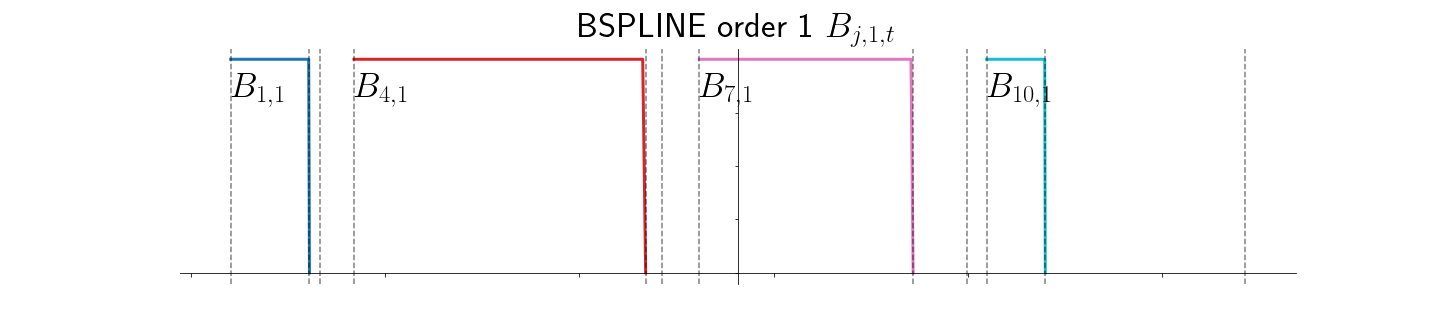
\includegraphics[width=\linewidth]{bspline_order_1.png}
	\caption{Some B-splines of order 1}\label{fig:bspline-order-1}
      \end{figure}
    \item \underline{$k=2$}
      \begin{align*}
        B_{j,2}(t) &= (t_{j+2}-t_j)\frac{[t_{j+1}, t_{j+2}]{(\cdot-t)}_+^1-[t_{j}, 
        t_{j+1}]{(\cdot-t)}_+^1}{t_{j+2}-t_j}\\
        &= \frac{{(t_{j+2}-t)}_+^1-{(t_{j+1}-t)}_+^1}{t_{j+2}-t_{j+1}}- 
        \frac{{(t_{j+1}-t)}_+^1-{(t_{j}-t)}_+^1}{t_{j+1}-t_{j}} \\
        &= 
        \begin{dcases}
	  \frac{t-t_j}{t_{j+1}-t_j} & t_j \leq t < t_{j+1},\\
	  \frac{t_{j+2}-t}{t_{j+2}-t_{j+1}} & t_{j+1} \leq t < t_{j+2}, \\
	0 & \mathrm{elsewhere}.
      \end{dcases}
      \end{align*}
      \begin{figure}[!h]
	\centering
	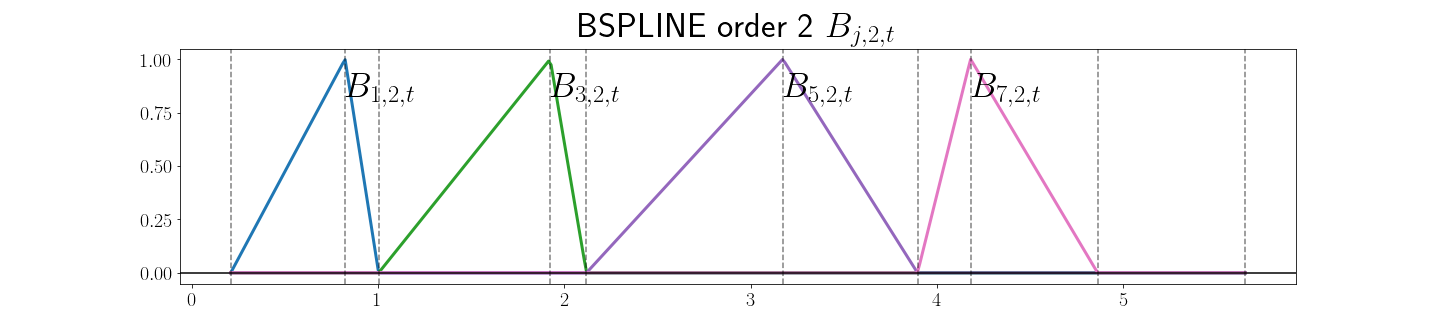
\includegraphics[width=\linewidth]{bspline_order_2.png}
	\caption{Some B-splines of order 2}\label{fig:bspline-order-2}
      \end{figure}
  \end{itemize}
\end{example}

\begin{remark}
  \begin{enumerate}
    \item Schoenberg also defined a general B-spline~\cite[Lecture 1, (2.1)]{schoenberg_cardinal_1973-1}) as
    \begin{equation*}
      M_{j,k,\bm{t}}(t) = k[t_j, \ldots, t_{j+k}]{(\cdot-t)}_+^{k-1}.
    \end{equation*}
    It is related to De Boor's general B-spline as
    \begin{equation*}
      \frac{k}{t_{j+k}-t_j}B_{j,k,\bm{t}},
    \end{equation*}
    which yields to the same definition provided that $t_{j+k} - t_j = k$.
  \item De Boor's \emph{B-splines} are the same as Schoenberg's forward B-splines (\ref{eq:fbspline})  when
    $\bm{t} = \mathbb{Z}$, i.e,
    \begin{equation*}
      B_{j,k,\mathbb{Z}}(t) = Q_k(t-j).
    \end{equation*}
  \end{enumerate}
\end{remark}

From the definition of B-splines in the most general case, a \emph{spline} is defined as follows
\begin{deftn}[{\cite[Chapter IX, (26)]{de_boor_practical_2001}}]\label{def:gen-splines}
  A spline function of order $k$ with knot sequence $\bm{t}$ is a linear combination of B-splines. $\mathscr{S}_{k, 
  \bm{t}}$ denotes the collection of all such splines, i.e,
  \begin{equation*}
    \mathscr{S}_{k, \bm{t}} := \{ \sum_{i=-\infty}^{\infty} c_i B_{i,k,\bm{t}} | \bm{c} \in \mathbb{R}^{\mathbb{Z}}\}
  \end{equation*}
\end{deftn}

\begin{remark}
  In the definition above, the sum is infinite while $\bm{t}$, and therefore the set $(B_{i, k,\bm{t}})$, may be finite 
  by assumption. When $\bm{t}$ is finite, choose $c_i=0$ for every $i$ where $B_{i,k,\bm{t}}$ is not defined. In the 
  properties given afterwards, we will voluntarily leave the limits of the sum unspecified. We could have restricted 
  ourselves to infinite sequences of knots $\bm{t}$, but it is an unnecessary limitation as all results hold for finite 
  sequences, albeit with different notations.
\end{remark}

As suggested in the subsection title, the approach used by De Boor mirrors that of Schoenberg.  Schoenberg first defines 
cardinal splines and then goes on to prove that cardinal B-splines form a basis for the collection formed by the 
cardinal splines. De Boor chooses to start by defining B-splines and later on defines splines as those functions that 
are written as linear combinations of B-splines. In the end, both definitions are equivalent, given 
Theorem~\ref{thm:curry-sch}, proposed by Curry and Schoenberg. Let us define the \textit{basic interval} $I_{k, \bm{t}}$  
as follows
\begin{equation*}
  I_{k, \bm{t}} = (t_-, t_+), \quad t_- := 
  \begin{dcases} t_k & \text{if} \ \bm{t} = (t_1, \ldots) \\ \inf t_j & \text{otherwise} \end{dcases}, 
  \quad t_+ := \begin{dcases} t_{n+1} & \text{if} \ \bm{t} = (\ldots, t_{n+k}) \\ \sup t_j & \text{otherwise} 
  \end{dcases}.
\end{equation*}
In the following proposition, we summarize the most useful properties of B-splines.
\begin{prop}[{\cite[Chapters IX, X, XI]{de_boor_practical_2001}}]
  \begin{enumerate}
    \item (Recurrence relation) \begin{equation*}
	B_{i,k} = \omega_{i,k} B_{i,k-1} + (1-\omega_{i+1,k})B_{i+1, k-1},
      \end{equation*}
      with
      \begin{equation*}
	\omega_{i,k}(t) = \frac{t-t_i}{t_{i+k-1}-t_i}.
      \end{equation*}
    \item (Marsden's identity)
      For any $\tau \in \mathbb{R}$, \begin{equation*}
	{(\cdot-\tau)}^{k-1} = \sum_{i} \psi_{i,k}(\tau) B_{i,k},
      \end{equation*}
      with 
      \begin{equation*}
	\psi_{i,k}(\tau) := (t_{i+1}-\tau)\cdots(t_{i+k-1}-\tau).
      \end{equation*}
    \item (Reproduction capabilities)
      From Marsden's identity,
      \begin{equation*}
	\Pi_{<k} \subset \mathscr{S}_{k, \bm{t}}.
      \end{equation*}
      In particular, $(B_{i,k})$ is a local partition of unity, i.e,
      \begin{equation*}
	\sum_{i} B_{i,k} = 1 \quad \mathrm{on} \ I_{k, \bm{t}}.
      \end{equation*}
    \item (Uniqueness and stability)
      There exists a positive constant $D_{k, \infty}$ independent of $\bm{t}$ such that
      \begin{equation*}
	\forall \bm{c} \in \mathbb{R}^{\mathbb{Z}}, \quad D_{k, \infty}^{-1} {\|\bm{c}\|}_{\infty} \leq {\left\| 
	\sum_{i} c_{i} B_{i,k} \right\|}_{\infty} \leq {\|\bm{c}\|}_{\infty}.
      \end{equation*}
  \end{enumerate}
\end{prop}
The spline space $\mathscr{S}_{k,\bm{t}}$ is finally completely characterized by the Curry-Schoenberg theorem, which 
also unveils its connection with piecewise-polynomial functions.
\begin{thm}[\cite{curry_polya_1966},{\cite[Chapter IX, (44)]{de_boor_practical_2001}}]\label{thm:curry-sch}
  Let $l \in \mathbb{N}^*$. For a given increasing sequence $\bm{\xi} = {(\xi_i)}_{i \in \llbracket1,l+1\rrbracket}$, 
  and a given nonnegative sequence of integers $\bm{\nu} = {(\nu_i)}_{i \in \llbracket2,l\rrbracket}$ with $\nu_i \leq  
  k$, set \begin{equation*}
    n := kl - \sum_{i=2}^{l} k - \nu_i = \dim \Pi_{<k, \bm{\xi}, \bm{\nu}}
  \end{equation*}
  and let $\bm{t} = {(t_i)}_{i \in \llbracket1,n+k\rrbracket}$ a nondecreasing sequence obtained from $\xi$ such that
  \begin{enumerate}
    \item for $i \in \llbracket2,l\rrbracket$, $\xi_i$ appears $k-\nu_i$ times in $\bm{t}$
    \item $t_1 \leq \ldots \leq t_k \leq \xi_1$ and $\xi_{l+1} \leq t_{n+1} \leq \ldots t_{n+k}$
  \end{enumerate}
  Then $B_{1,k}, \ldots, B_{n,k}$ is a basis for $\Pi_{k, \xi, \nu}$ on $I_{k,t} = [t_k,t_{n+1}]$, i.e,
  \begin{equation*}
    {\mathscr{S}_{k, \bm{t}}}_{|I_{k,t}} = {\Pi_{<k, \bm{\xi}. \bm{\nu}}}_{|I_{k,t}}.
  \end{equation*}
\end{thm}
